% Type of the document
\documentclass{beamer}

% elementary packages:
\usepackage{graphicx}
\usepackage[latin1]{inputenc}
\usepackage[T1]{fontenc}
\usepackage[english]{babel}
\usepackage{listings}
\usepackage{xcolor}
\usepackage{eso-pic}
\usepackage{mathrsfs}
\usepackage{url}
\usepackage{amssymb}
\usepackage{amsmath}
\usepackage{multirow}
\usepackage{hyperref}
\usepackage{booktabs}
\usepackage{tikz}
\usepackage{graphicx}
\usepackage{subfig}



% additional packages
\usepackage{bbm}

% packages supplied with ise-beamer:
\usepackage{cooltooltips}
\usepackage{colordef}
\usepackage{beamerdefs}
\usepackage{lvblisting}

% Mathematics
\usepackage{amssymb}
\usepackage{amsmath}
\usepackage{mathrsfs}
\usepackage{amsthm,amsfonts}
\usepackage{mathtools}
\usepackage{algorithmic}
\usepackage[linesnumbered,ruled]{algorithm2e}
\usepackage{float}

\usepackage{copyrightbox}


% Change the pictures here:
% logobig and logosmall are the internal names for the pictures: do not modify them. 
% Pictures must be supplied as JPEG, PNG or, to be preferred, PDF
\pgfdeclareimage[height=2cm]{logobig}{Figures/hulogo}
% Supply the correct logo for your class and change the file name to "logo". The logo will appear in the lower
% right corner:
\pgfdeclareimage[height=0.7cm]{logosmall}{Figures/hulogo}

% Title page outline:
% use this number to modify the scaling of the headline on title page
\renewcommand{\titlescale}{1.0}
% the title page has two columns, the following two values determine the percentage each one should get
\renewcommand{\titlescale}{1.0}
\renewcommand{\leftcol}{0.6}

% smaller font for selected slides
\newcommand\Fontvi{\fontsize{10}{7.2}\selectfont}
\newcommand\Fontsm{\fontsize{8}{7.2}\selectfont}


% Define the title. Don't forget to insert an abbreviation instead 
% of "title for footer". It will appear in the lower left corner:
\title[ABC]{Approximative Bayesian Computation}
% Define the authors:
\authora{Jost von Petersdorff-Campen} % a-c
\authorb{}
\authorc{}

% Define any internet addresses, if you want to display them on the title page:
\def\linka{}
\def\linkb{}
\def\linkc{}
% Define the institute:
\institute{Chair of Applied Statistics \\
Humboldt--Universit{\"a}t zu Berlin \\}

% Comment the following command, if you don't want, that the pdf file starts in full screen mode:
\hypersetup{pdfpagemode=FullScreen}


\newcommand\Wider[2][3em]{%
\makebox[\linewidth][c]{%
  \begin{minipage}{\dimexpr\textwidth+#1\relax}
  \raggedright#2
  \end{minipage}%
  }%
}


%%%%
% Main document
%%%%
\begin{document}
\captionsetup[figure]{labelformat=empty}
\long\def\/*#1*/{}

% Draw title page
\frame[plain]{%
\titlepage{}
}

% The titles of the different sections of you talk, can be included via the \section command. The title will be displayed in the upper left corner. To indicate a new section, repeat the \section command with, of course, another section title
%%%%%%%%%%%%%%%%%%%%%%%%%%%%%%%%%%%%%%%%%%%%%%%%%%%%%%%%%%%%%%%%%%%%%%%%%%%%%%%%%%%%%%%%%%%%%%%%%%%%%%%%%%%%%%%%%%%%%%%%
%%%%%%%%%%%%%%%%%%%%%%%%%%%%%%%%%%%%%%%%%%%%%%%%%%%%%%%%%%%%%%%%%%%%%%%%%%%%%%%%%%%%%%%%%%%%%%%%%%%%%%%%%%%%%%%%%%%%%%%%


\section{Introduction}
%%%%%%%%%%%%%%%%%%%%%%%%%%%%%%%%%%%%%%%%%%%%%%%%%%%%%%%%%%%%%%%%%%%%%%%%%%%%%%%%%%%%%%%%%%%%%%%%%%%%%%%%%%%%%%%%%%%%%%%%

\frame{
\frametitle{Motivation}
\begin{align*}
p(\theta|y_{obs}) \propto p(y_{obs}|\theta)p(\theta)
\end{align*}
\begin{itemize}
\item Basic requirement for inference: The Likelihood
\item However, sometimes the Likelihood...\\
\begin{itemize}
\item ... is costly to evaluate
\item ... has no closed-form
\item ... is actually unknown
\end{itemize} 

\end{itemize}
}

\frame{
\frametitle{}
\textbf{Idea}: Generate a joint sample $(\theta,y)$ and condition on $y_{obs}$ to get a sample from the posterior.\\
\bigskip
We know:
\begin{equation*}
p(\theta|y_{obs}) \propto p(y_{obs}|\theta)p(\theta) \color{blue}=  p(\theta,y=y_{obs})
\end{equation*}


}

\frame{
\frametitle{}
\begin{algorithm}[H]
\SetAlgoLined
\KwResult{Sample from the posterior}
 initialization:  M iterations \\
 \For{m=1:M}{
   Sample $\theta_m$ from $p(\theta)$\\
   Simulate $y_m$ from $p(y|\theta_m)$  \\
   accept $\theta_m$ if $y_m=y_{obs}$  \\         
 \caption{Basic ABC}}
\end{algorithm}
}

\section{Discrete}

\frame{
\frametitle{Discrete Example}
$p(\theta) \sim B(1,1)$ ; $y|\theta \sim bin(10,\theta)$ ; $y_{obs}=7$; sample: $20.000$
\begin{center}
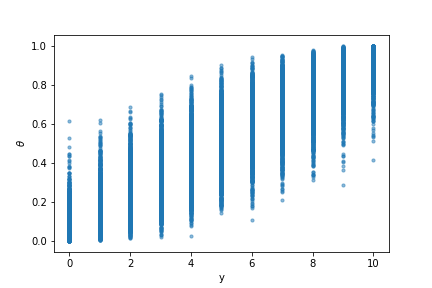
\includegraphics[scale=0.5]{Figures/discrete.png}

\end{center}

}
\frame{
\frametitle{Discrete Example}
$p(\theta) \sim B(1,1)$ ; $y|\theta \sim bin(10,\theta)$ ; $y_{obs}=7$; sample: $20.000$
\begin{center}
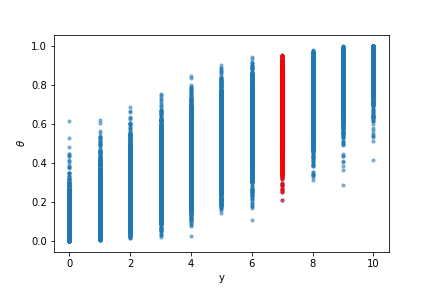
\includegraphics[scale=0.5]{Figures/discrete2.png}

\end{center}

}

\frame{
\frametitle{Discrete Example}
$p(\theta) \sim B(1,1)$ ; $y|\theta \sim bin(10,\theta)$ ; $y_{obs}=7$; sample: $20.000$
\begin{center}
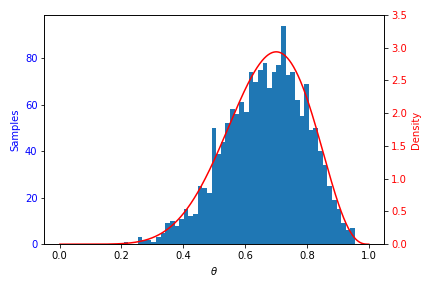
\includegraphics[scale=0.5]{Figures/histogram_dens.png}

\end{center}

}

\section{Continuous}

\frame{
\frametitle{Continuous Example}
$p(\theta) \sim N(0,1)$; $y|\theta \sim N(\theta ,1)$; $y_{obs}=1$; sample: $20.000$

\begin{center}

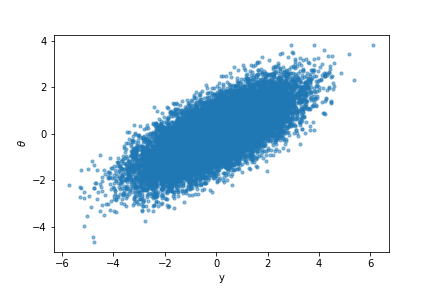
\includegraphics[scale=0.5]{Figures/scatter_cont.png}
\end{center}

}

\frame{
\frametitle{Replace exact inference with "good enough"}
\begin{algorithm}[H]
\SetAlgoLined
\KwResult{Sample from the posterior $p_{\epsilon}(\theta|y_{obs})$}
 initialization:  M iterations, $\epsilon$, distance measure $d(.,.)$ \\
 \For{m=1:M}{
   Sample $\theta_m$ from $p(\theta)$\\
   Simulate $y_m$ from $p(y_{obs}|\theta_m)$  \\
   accept $\theta_m$ if $d(y_m,y_{obs})<\epsilon$  \\         
 \caption{Basic ABC with $\epsilon$}}
\end{algorithm}

}

\frame{
\frametitle{}
$\epsilon=0.3$
\begin{figure}[ht] 
  \begin{minipage}[l]{0.5\linewidth}
		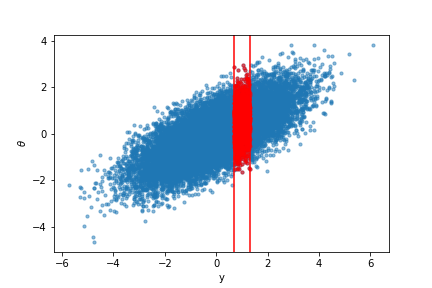
\includegraphics[scale=0.35]{Figures/scatter_cont_eps.png} \end{minipage}\begin{minipage}[r]{0.5\linewidth}
		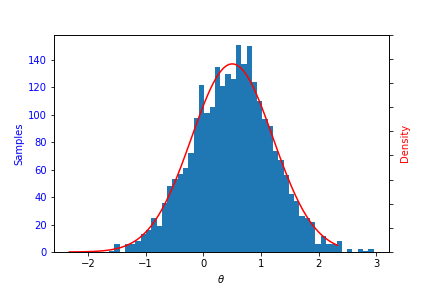
\includegraphics[scale=0.35]{Figures/cont_dens_hist.png}
  \end{minipage}
 \end{figure}

}


\frame{
\frametitle{}
What if we choose a too tiny $\epsilon$?

\begin{figure}[ht] 
  \begin{minipage}[l]{0.5\linewidth}
		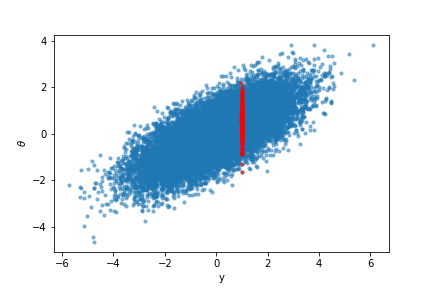
\includegraphics[scale=0.35]{Figures/cont_scatter_tiny_eps.png} \end{minipage}\begin{minipage}[r]{0.5\linewidth}
		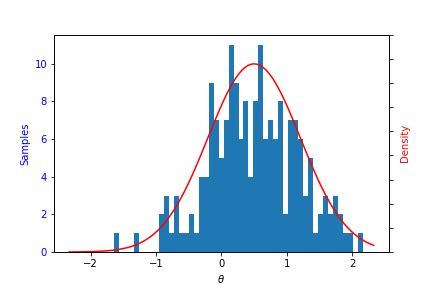
\includegraphics[scale=0.35]{Figures/cont_dens_hist_compare2.png}
  \end{minipage}
 \end{figure}


}








\frame{
\frametitle{}
What if we choose a too big $\epsilon$?

\begin{figure}[ht] 
  \begin{minipage}[l]{0.5\linewidth}
		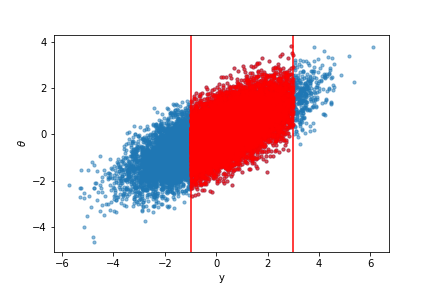
\includegraphics[scale=0.35]{Figures/cont_scatter_wide_eps.png} \end{minipage}\begin{minipage}[r]{0.5\linewidth}
		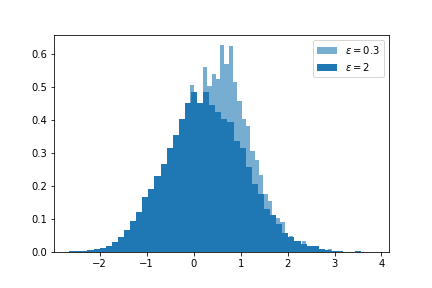
\includegraphics[scale=0.35]{Figures/cont_dens_hist_compare.png}
  \end{minipage}
 \end{figure}


}


\section{Kernel}
\frame{
\frametitle{}
Use a Kernel to prevent the this shift $\rightarrow$ Accept draws with a probability proportional to the distance. 

\begin{figure}[ht] 
  \begin{minipage}[l]{0.5\linewidth}
		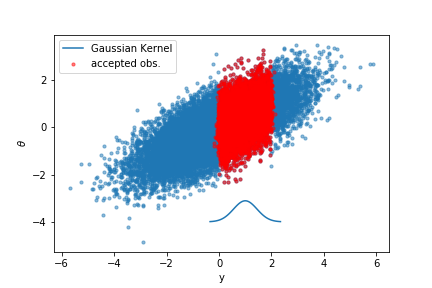
\includegraphics[scale=0.35]{Figures/cont_scatter_kernel.png} \end{minipage}\begin{minipage}[r]{0.5\linewidth}
		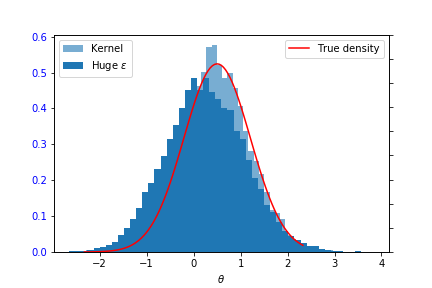
\includegraphics[scale=0.35]{Figures/cont_dens_hist_kernel_eps.png}
  \end{minipage}
 \end{figure}

\center\color{blue}Assumption: $p(\theta|y_{obs}) \approx p_{\epsilon}(\theta|y_{obs})$

}
\section{Summary statistics}
\frame{
\frametitle{}
This alll works fine with just one observation.\\
\bigskip
\textbf{But:} With $y_{obs}=(y_{obs,1},...,y_{obs,n})$ evaluating $d(y_{obs},y_m)$ in every step is very costly and suffers from the \textbf{Curse of Dimensionality}!

}

%%%%%%%%%%%%%%%%%%%%%%%%%%%%%%%%%%%%%%%%%%%%%%%%%%%%%%%%%%%%%%%%%%%%%%%%%%%%%%%%%%%%%%%%%%%%%%

\frame{
\frametitle{Summary Statistics}

\textbf{Solution:} Use summary statistics to map data to a lower dimension without losing too much information.\\
\bigskip 

Sufficient Statistic (heuristically): "A statistic satisfies the criterion of sufficiency when no other statistic which can be calculated from the same sample provides any additional information"\cite{fisher1922mathematical}

\bigskip 

$X=X_1,...,X_n$ independent uniformly distributed on $[0,\theta]$.
What is a sufficient $s(X)$?

}


\frame{
\frametitle{Summary Statistics}

\textbf{Solution:} Use summary statistics to map data to a lower dimension without losing too much information.\\
\bigskip 

Sufficient Statistic (heuristically): "A statistic satisfies the criterion of sufficiency when no other statistic which can be calculated from the same sample provides any additional information"\cite{fisher1922mathematical}

\bigskip 

$X=X_1,...,X_n$ independent uniformly distributed on $[0,\theta]$.
What is a sufficient $s(X)$? \textbf{Solution: $s(X)=max(X_1,...,X_n)$} 

}

%%%%%%%%%%%%%%%%%%%%%%%%%%%%%%%%%%%%%%%%%%%%%%%%%%%%%%%%%%%%%%%%%%%%%%%%%%%%%%%%%%%%%%%%%%%%%%%%

\frame{
\frametitle{Again: Replace exact inference with "good enough"}

Using sufficient summary statistics yields exact inference, but rarely exist  in real applications. \\
\bigskip
Find a summary statistic that maximizes the trade-off of reducing dimensionality and losing information $\leftarrow$ model dependent

\center\color{blue}Assumption: $p(\theta|y_{obs}) \approx p(\theta|s_{obs})$
}

%%%%%%%%%%%%%%%%%%%%%%%%%%%%%%%%%%%%%%%%%%%%%%%%%%%%%%%%%%%%%%%%%%%%%%%%%%%%%%%%%%%%%%%%%%%%%%%%
\frame{
\frametitle{}
\begin{algorithm}[H]
\SetAlgoLined
\KwResult{Sample from the posterior $p_{\epsilon}(\theta|s_{obs})$}
 initialization:  M iterations, $\epsilon$, distance measure $d(.,.)$, Kernel $K$ \\
 \For{m=1:M}{
    Sample  $\theta_i$ from  $p(\theta)$\\
Simulate $s_i$ from $p(s|\theta_i)$\\
accept $\theta_i$ with probability proportional to $K_{\epsilon}(d(s_i,s_{obs}))$\\
 \caption{ABC}}
\end{algorithm}

}


    
\section{Further refinement}               

\frame{
\frametitle{Regression adjustment}
\textbf{Motivation:} Adjust for discrepancy of simulations and observations. 
Estimating the posterior is estimating a conditional density. \\
$\rightarrow$ suggests Regression!
\bigskip
\begin{itemize}

\item 
$\theta_i = \beta_0 + \beta^\intercal (s_i-s_{obs})+\eta_i$, \text{ with $\eta_i$ i.i.d. and mean zero}
\item if $s_i=s_{obs}$ $\rightarrow$ $\theta_i$ is drawn from posterior with $E[\theta|s]=\beta_0$ 
\item $\theta_i^*=\theta_i-\hat{\beta}^T(s_i-s_{obs})=\hat{\beta_0}+\hat{\eta_i}$
\end{itemize}
\bigskip

$\rightarrow$ Lowers the sensitivity to the bandwidth $\epsilon$.\\
Can be further improved with nonlinear regression or local linear regression.



}

%\frame{
%\frametitle{Automation of choice of summary statistics}
%E.g. choose subset of summary statistics and test for sufficiency, \textbf{but:} Choice of summary statistics cannot be fully automized, since this depends on your belief on the data structure \cite{nott123}
%}


\frame{
\frametitle{ABC-MCMC}
Why? If data is informative (posterior more dense than the prior), just sampling values from the prior is inefficient. \\

\textbf{Idea}: Draw $\theta$ from a distribution which adaptively comes closer to the posterior.

}

\/*
\frame{

\begin{algorithm}[H]
\SetAlgoLined
\KwResult{sample of $p(\theta|s)$}
 initialization: $\epsilon$; M iterations; proposal density $q(.|\theta)$; $\theta^{(1)}$ \\
 \For{t=1:M}{
   Sample $\theta'$ from $q(.|\theta^{(t)})$\\
   Simulate $s$ from $f_n(s|\theta')$\\
   Draw $u$ from $U_{[0,1]}$\\
   Calculate $\alpha=min\{1,\frac{p(\theta')q(\theta^{(t)}|\theta')}{p(\theta^{(t)})q(\theta'|\theta^{(t)})} \mathbbm{1}\{||s-s_{obs}||\leq\epsilon\}\}$\\
   
  \eIf{$\alpha>u$}{
  Set $\theta^{(t+1)}=\theta'$
   }{
  Set $\theta^{(t+1)}=\theta^{(t)}$	
	  }
 }
 \caption{ABC-MCMC}
\end{algorithm} 
}

*/



\section{Application}
\frame{
\frametitle{Application to a predator-prey model}
\textbf{Motivation}: Explain shift of vole abundance through population of their predators (weasels). \\\cite{turchin2000living}, \cite{fasiolo2015approximate}, \cite{klein2019marginally}  \\

\begin{figure}[ht] 
  \begin{minipage}[l]{0.5\linewidth}
		\copyrightbox[b]{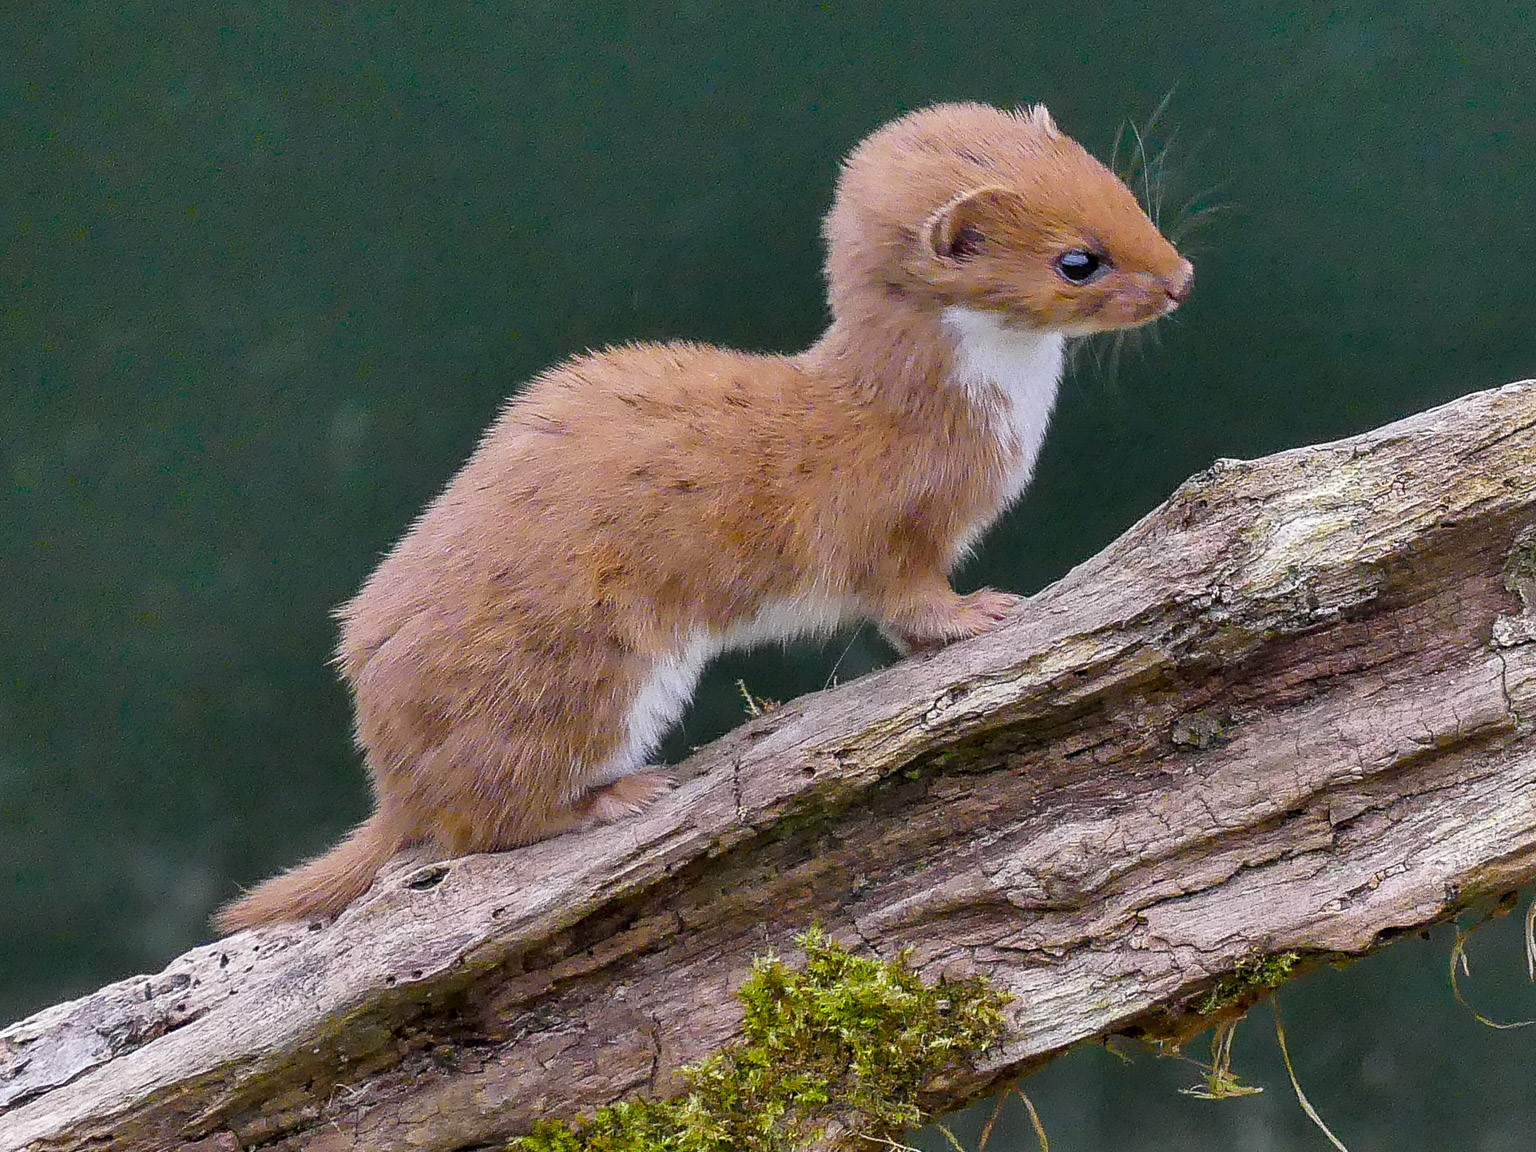
\includegraphics[scale=0.12]{Figures/weasel.jpg}}
		{Source: Mike Prince, https://www.flickr.com/photos/}	
		 \end{minipage}\begin{minipage}[r]{0.5\linewidth}
		\copyrightbox[b]{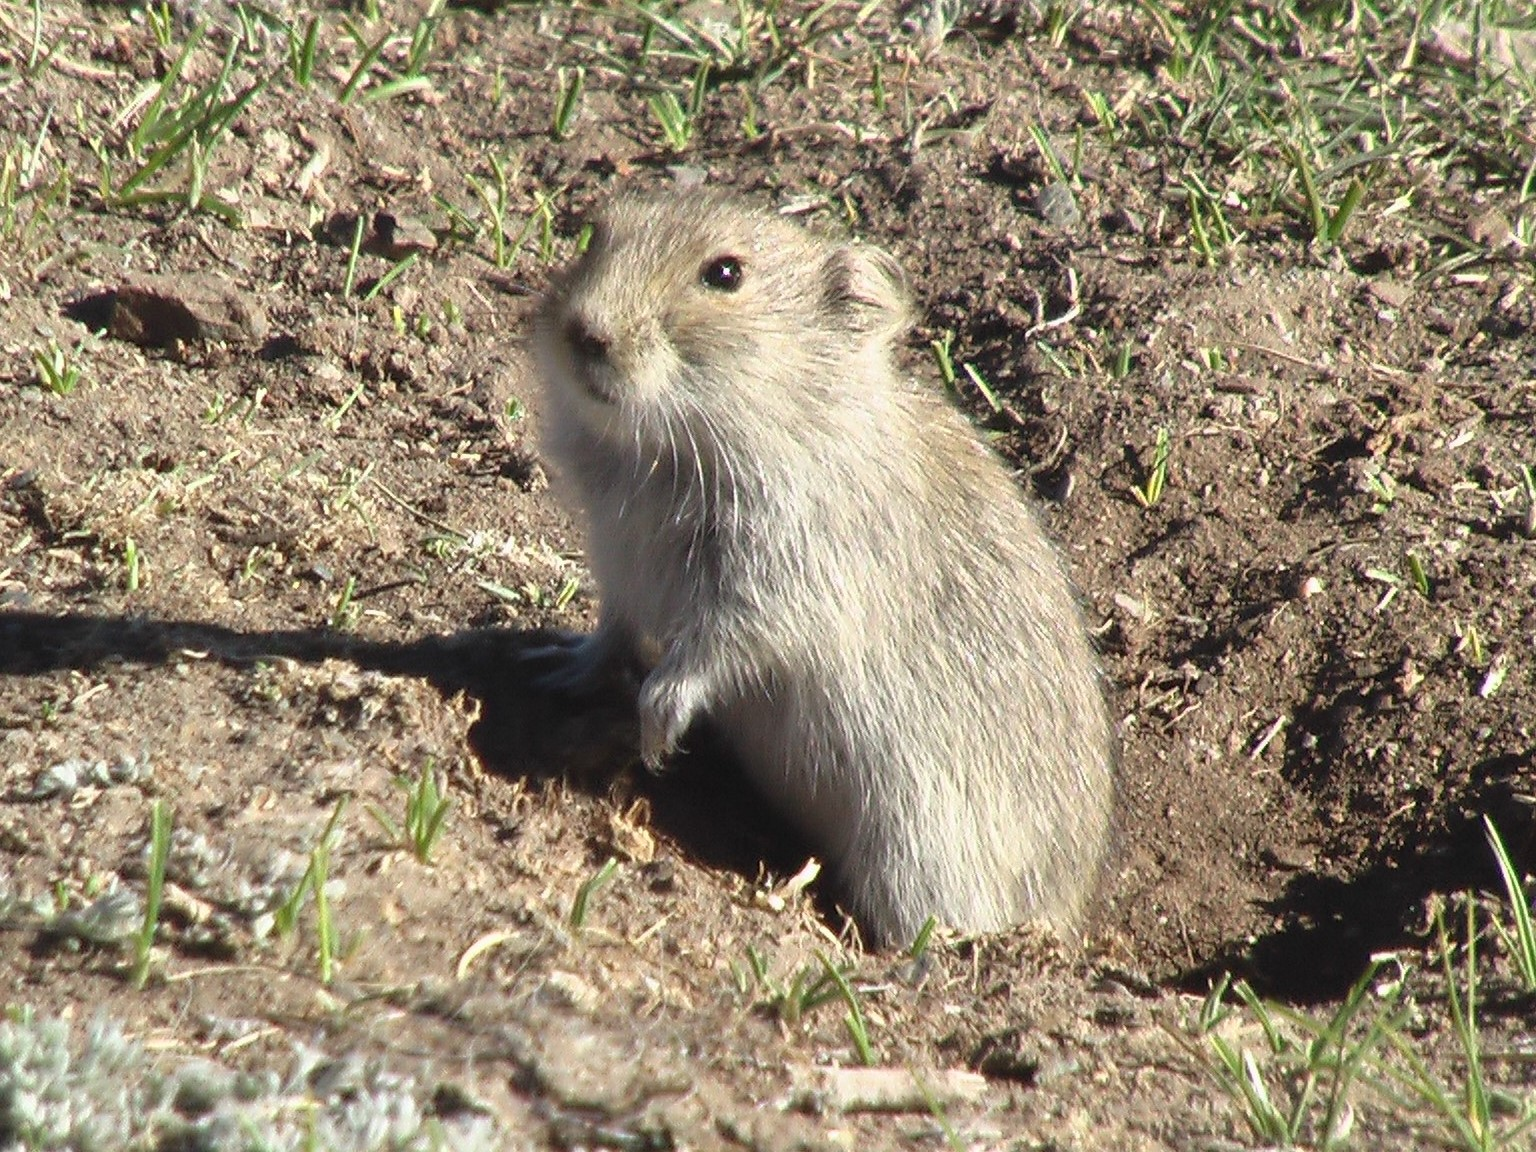
\includegraphics[scale=0.12]{Figures/vole.jpg}}
		{Source:Bogomolov.PL , via Wikimedia Commons}	
  \end{minipage}
 \end{figure}
}

\frame{

\textbf{Model}:
\begin{enumerate}
\item $\frac{dN}{dt}=r(1-esin2\pi t)N-\frac{r}{K}N^2-\frac{GN^2}{N^2+H^2}-\frac{CNP}{N+D}+\frac{N}{K}\frac{dw}{dt}$ 
\item $\frac{dP}{dt}=s(1-esin2\pi t)P-sQ\frac{P^2}{N}$
\end{enumerate}
\begin{itemize}
\item$N,P$ vole and weasle abundance, respectively.\\

\item $r,s$ intrinsic population growth rates.\\

\item $K$ Carrying capacity of voles.\\
\item $G$ Mortality inflicted of generalist hunters.

\end{itemize}
}


\frame{

\textbf{Model}:
\begin{enumerate}
\item $\frac{dN}{dt}=r(1-esin2\pi t)N-\frac{r}{K}N^2-\frac{GN^2}{N^2+H^2}-\frac{CNP}{N+D}+\frac{N}{K}\frac{dw}{dt}$ 
\item $\frac{dP}{dt}=s(1-esin2\pi t)P-sQ\frac{P^2}{N}$
\end{enumerate}
\begin{itemize}
\item $dw(t_2)-dw(t_1) \sim N(0,\sigma^2(t_2-t_1))$ Brownian motion process
\item $H$ is the half-saturation parameter
\item $Q$ number of voles needed for one weasel
\item $Y_t \sim Pois(\Phi N_t)$
\end{itemize}


}

\frame{
\frametitle{Data}

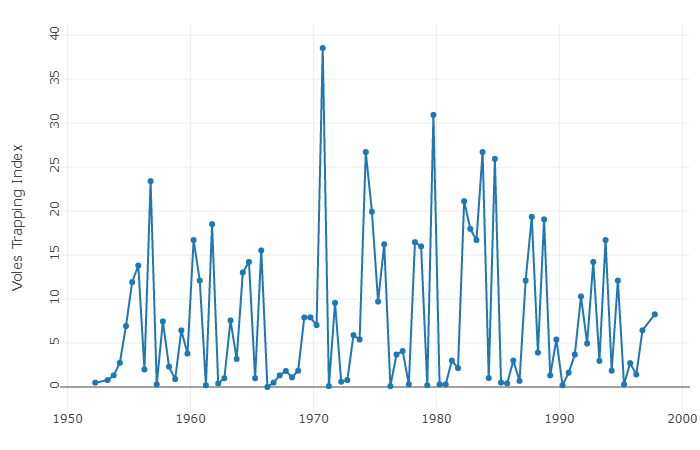
\includegraphics[scale=0.35]{Figures/voles.png}

}


%\frame{
%\frametitle{Why use ABC here?}
%\begin{itemize}
%\item Conditional dependencies between states at different time points
%\item Weasel abundance is hidden state

%\end{itemize}
%\bigskip


%$\rightarrow$ difficult calculation of the likelihood. \\




%}




\frame{
\frametitle{Priors \& Summary Statistics}
\Wider[4em]{
\begin{minipage}[l]{0.4\linewidth}
\begin{footnotesize}



\begin{table}
\begin{tabular}{c | c}
Parameter & Prior \\
\cline{1-2}\\
$r$ & $N(5,1)$\\
$e$ & $N(1,1)$\\
$g$ & $Exp(\lambda=7)$\\
$h$ & $Gamma(\eta=4,\theta=40)$\\
$a$ & $N(15,15)$\\
$d$ & $N(0.04,0.04)$\\
$s$ & $N(1.25,0.5)$\\
$\sigma$ & $Unif(0.5,\infty)$\\
$\phi$ & $Unif(0,\infty)$\\
\end{tabular}

\end{table}
\end{footnotesize}
\end{minipage}
\hspace{0.5cm}
 \begin{minipage}[r]{0.5\linewidth}
 \begin{flushright}
	\begin{itemize}
	\item autcovariances of $y_1,...,y_T$ up to lag 5
	\item mean population $\bar{y}-\tilde{y}$
	\item coefficients of the regression $y_{t+1}=\beta_1y_t+\beta_2y_t^2+\beta_3y_{t-6}+\beta_4y_{t-6}^2+\beta_5y_{t-6}^3$
	\item number of turning points
	\end{itemize}
 \end{flushright}
\end{minipage}
}

}





\frame{
  \frametitle{Results}
  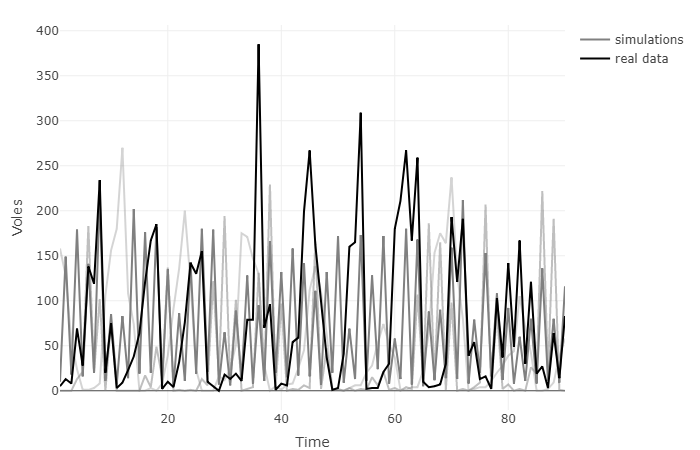
\includegraphics[scale=0.35]{Figures/voles_and_sim.png}
}

\frame{
  \frametitle{Results}
\begin{figure}[ht] 
  \begin{minipage}[l]{0.3\linewidth}
		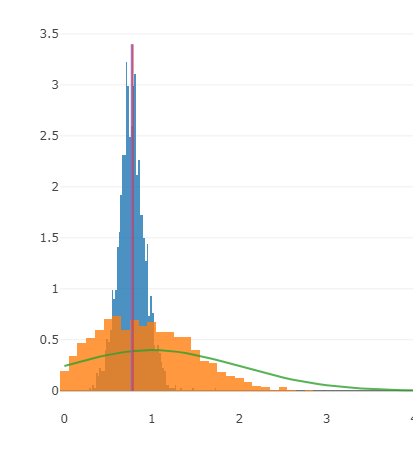
\includegraphics[scale=0.38]{Figures/e_both.png}
		\caption{\color{blue}e}		
		 \end{minipage}\begin{minipage}[r]{0.5\linewidth}
		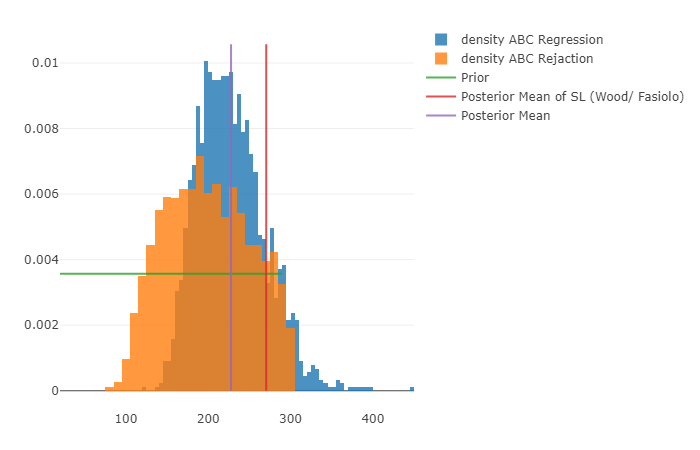
\includegraphics[scale=0.38]{Figures/phi_both.png}
		\caption{\color{blue}$\phi$}
  \end{minipage}
 \end{figure}
}


\/*
\frame{
  \frametitle{Results (Simple Rejection)}
  \begin{figure}[htbp]
  \captionsetup[subfloat]{labelformat=empty}
  % \centering
  \subfloat[r]{{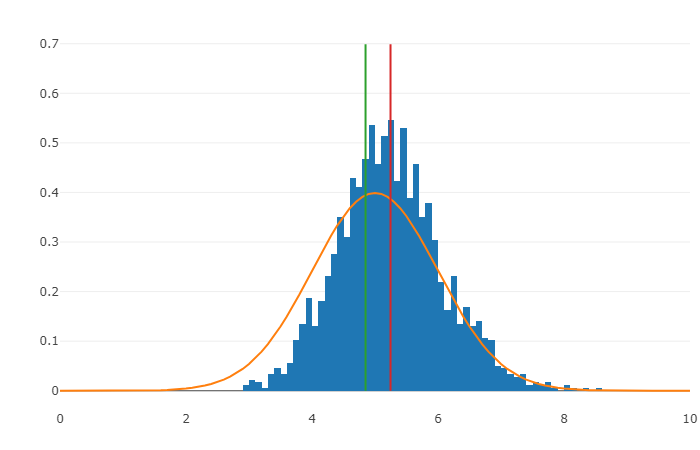
\includegraphics[width=0.33\textwidth]{Figures/r.png}}}
  \subfloat{{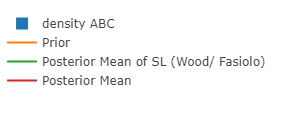
\includegraphics[width=0.33\textwidth]{Figures/legend.png}}}
  \\
  \subfloat[e]{{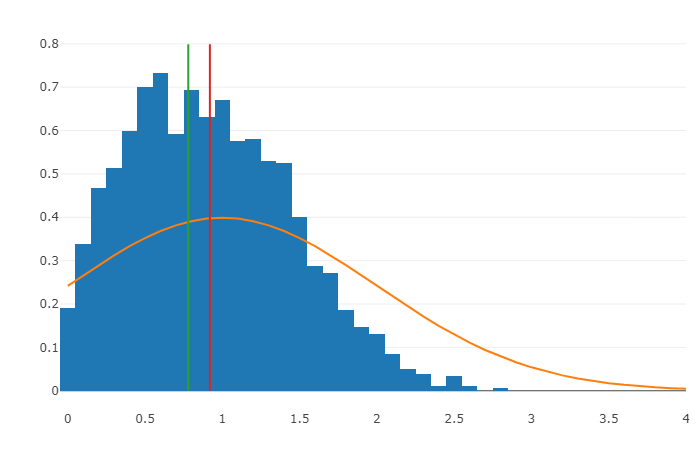
\includegraphics[width=0.33\textwidth]{Figures/e.png}}}
  \subfloat[g]{{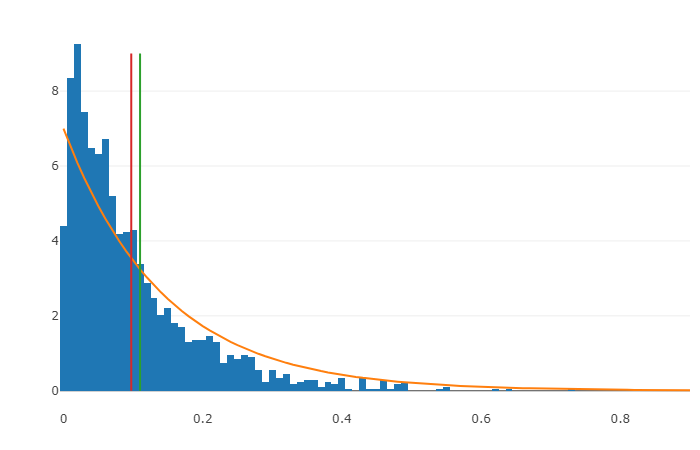
\includegraphics[width=0.33\textwidth]{Figures/g.png}}}
  
  
  \end{figure}
}



\frame{
  \frametitle{Results (Simple Rejection)}
  \begin{figure}[htbp]
  \captionsetup[subfloat]{labelformat=empty}
  % \centering
  \subfloat[h]{{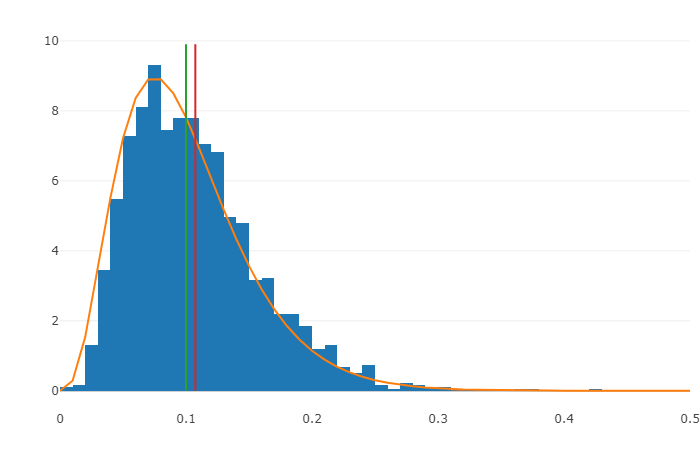
\includegraphics[width=0.33\textwidth]{Figures/h.png}}}
  \subfloat{{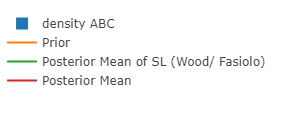
\includegraphics[width=0.33\textwidth]{Figures/legend.png}}}
  \\
  \subfloat[a]{{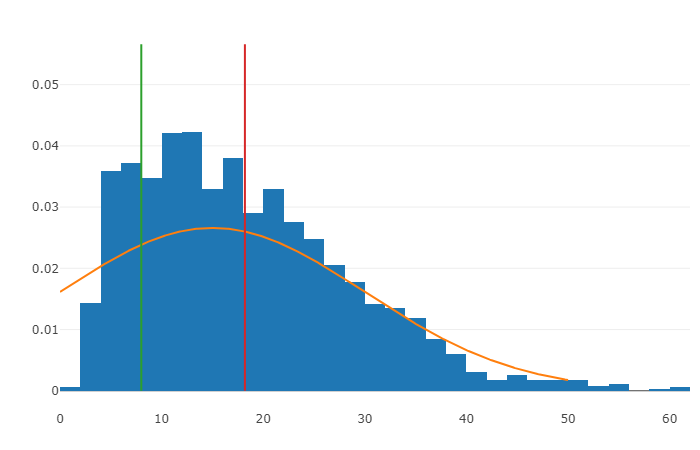
\includegraphics[width=0.33\textwidth]{Figures/a.png}}}
  \subfloat[d]{{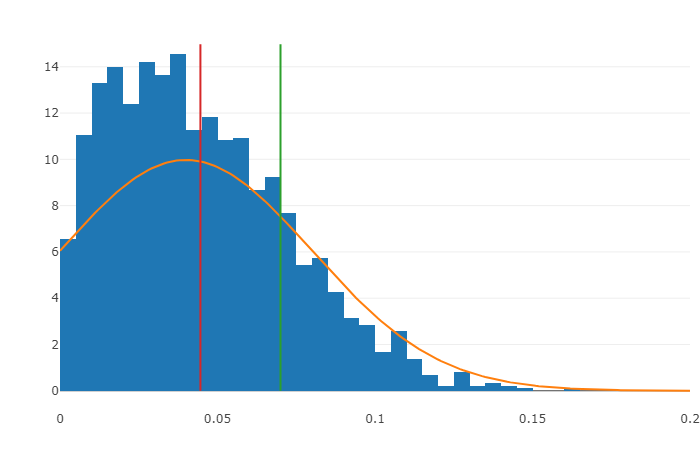
\includegraphics[width=0.33\textwidth]{Figures/d.png}}}
  
  
  \end{figure}
}




\frame{
  \frametitle{Results (Simple Rejection)}
  \begin{figure}[htbp]
  \captionsetup[subfloat]{labelformat=empty}
  % \centering
  \subfloat[s]{{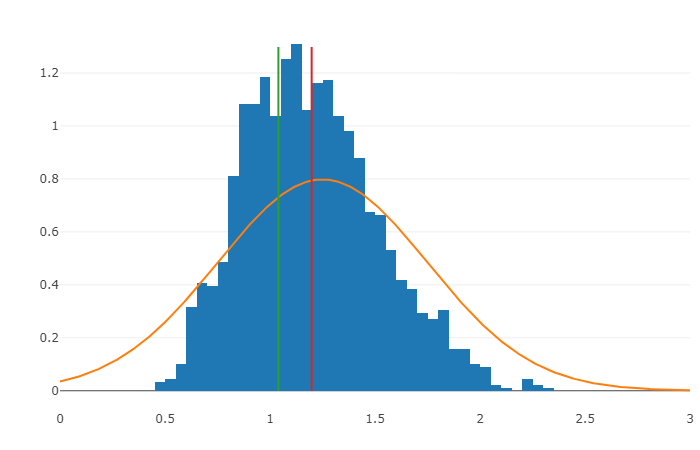
\includegraphics[width=0.33\textwidth]{Figures/s.png}}}
  \subfloat{{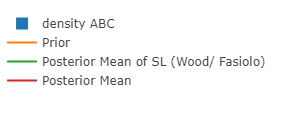
\includegraphics[width=0.33\textwidth]{Figures/legend.png}}}
  \\
  \subfloat[$\sigma$]{{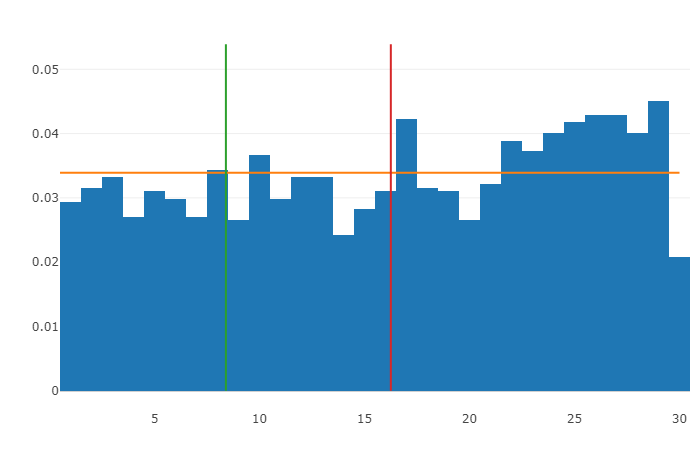
\includegraphics[width=0.33\textwidth]{Figures/sigma.png}}}
  \subfloat[$\phi$]{{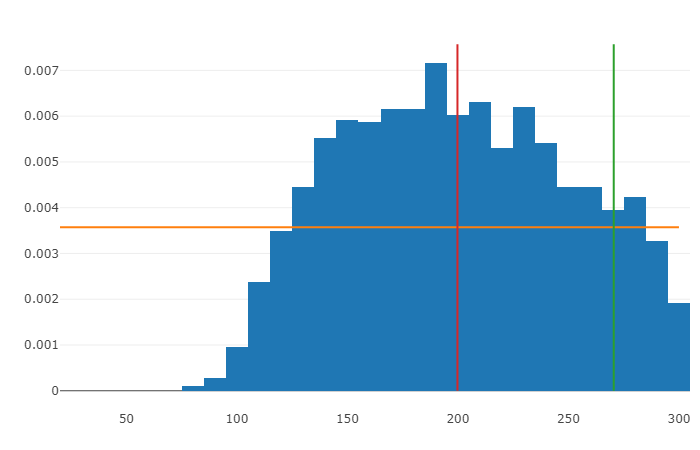
\includegraphics[width=0.33\textwidth]{Figures/phi.png}}}
  
  
  \end{figure}
}

\frame{
  \frametitle{Results (Regression Adjustment)}
  \begin{figure}[htbp]
  \captionsetup[subfloat]{labelformat=empty}
  % \centering
  \subfloat[r]{{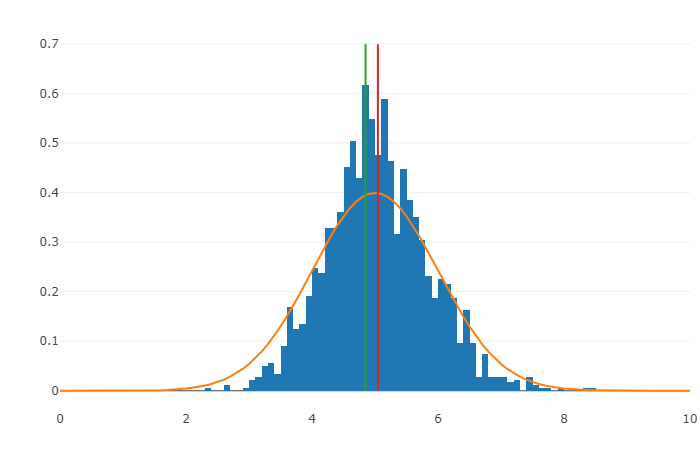
\includegraphics[width=0.33\textwidth]{Figures/r_lin.png}}}
  \subfloat{{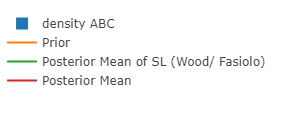
\includegraphics[width=0.33\textwidth]{Figures/legend.png}}}
  \\
  \subfloat[e]{{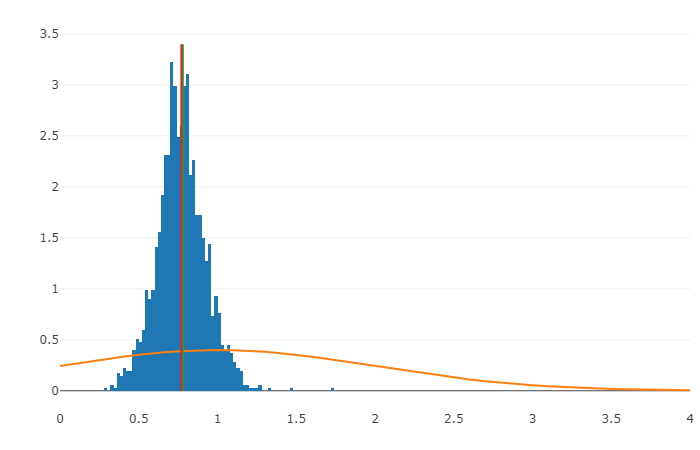
\includegraphics[width=0.33\textwidth]{Figures/e_lin.png}}}
  \subfloat[g]{{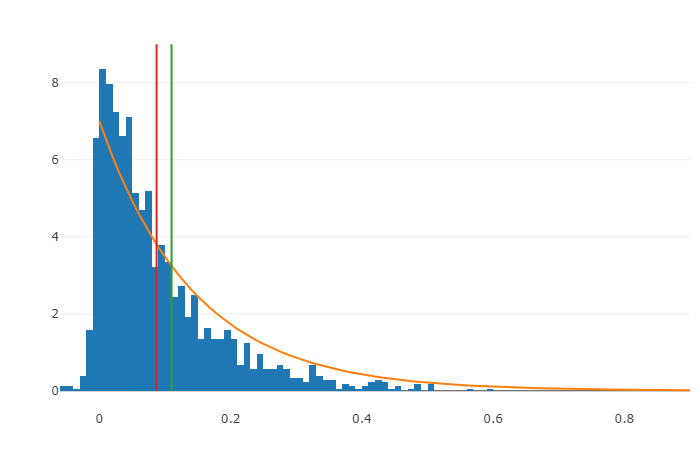
\includegraphics[width=0.33\textwidth]{Figures/g_lin.png}}}
  
  
  \end{figure}
}



\frame{
  \frametitle{Results (Regression Adjustment)}
  \begin{figure}[htbp]
  \captionsetup[subfloat]{labelformat=empty}
  % \centering
  \subfloat[h]{{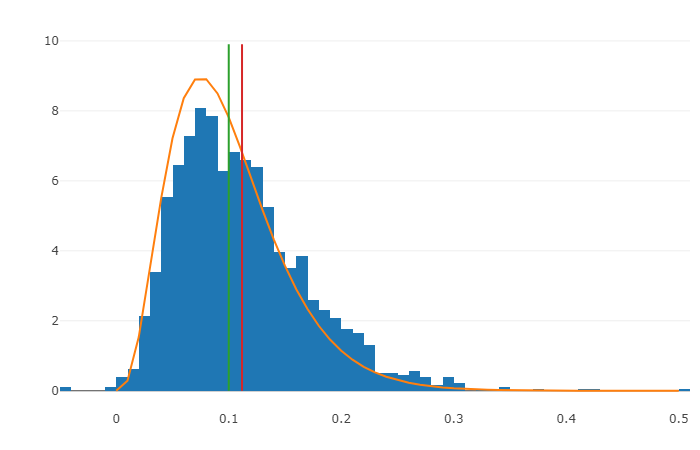
\includegraphics[width=0.33\textwidth]{Figures/h_lin.png}}}
  \subfloat{{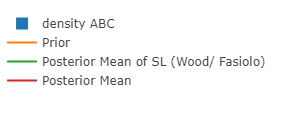
\includegraphics[width=0.33\textwidth]{Figures/legend.png}}}
  \\
  \subfloat[a]{{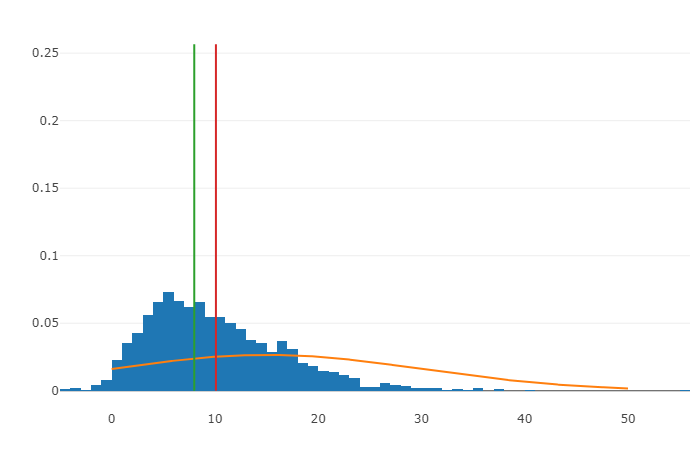
\includegraphics[width=0.33\textwidth]{Figures/a_lin.png}}}
  \subfloat[d]{{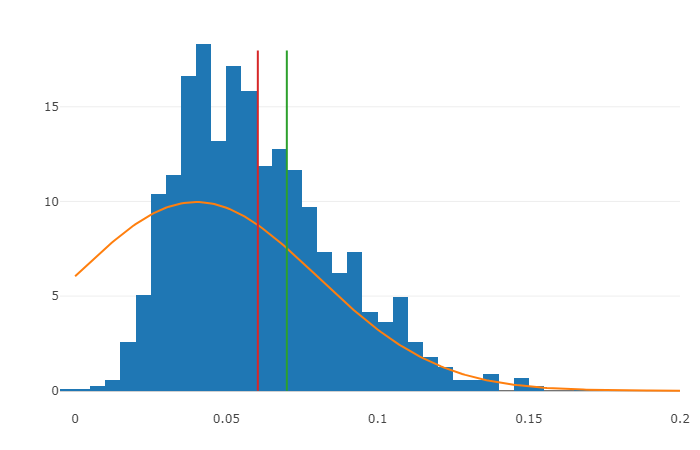
\includegraphics[width=0.33\textwidth]{Figures/d_lin.png}}}
  
  
  \end{figure}
}




\frame{
  \frametitle{Results (Regression Adjustment)}
  \begin{figure}[htbp]
  \captionsetup[subfloat]{labelformat=empty}
  % \centering
  \subfloat[s]{{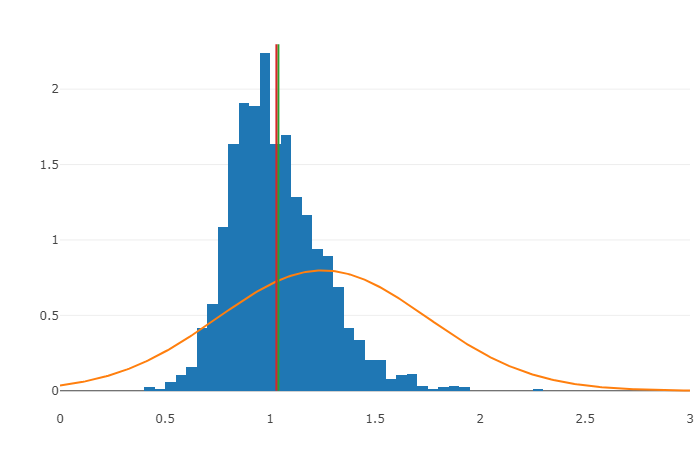
\includegraphics[width=0.33\textwidth]{Figures/s_lin.png}}}
  \subfloat{{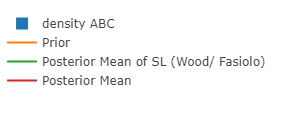
\includegraphics[width=0.33\textwidth]{Figures/legend.png}}}
  \\
  \subfloat[$\sigma$]{{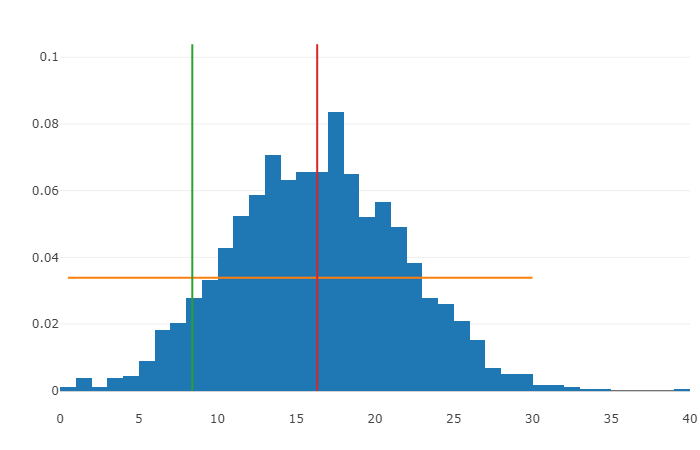
\includegraphics[width=0.33\textwidth]{Figures/sigma_lin.png}}}
  \subfloat[$\phi$]{{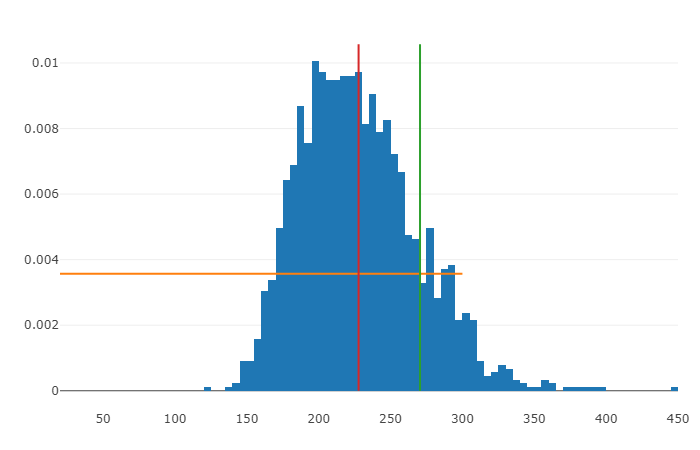
\includegraphics[width=0.33\textwidth]{Figures/phi_lin.png}}}
  
  
  \end{figure}
}

*/

\frame{
\frametitle{Performance}
\begin{itemize}
\item Assume pseudo true parameters and create multiple fake data sets
\item Run \textit{ABC} on each of the fake data sets
\item Measure \textit{Mean Squared Error} of the estimate
\end{itemize}
}

\frame{
\frametitle{Performance}
15 data sets; 10.000 iterations per set; acceptance rate$=0.1$
\begin{footnotesize}



\begin{table}
\begin{tabular}{c | c | c | c | c | c}
 &  &  \multicolumn{2}{c}{Mean of Posterior means} & \multicolumn{2}{c}{RMSE} \\
\cline{3-6}

   Parameter & Value & Rejection & Regression & Rejection & Regression \\
\hline
$r$ & 5 &  5.42  		& 5.46&		0.42  	&0.46 \\
$e$ & 1.58 & 1.88   	&   1.89& 		0.30    & 0.31  \\
$g$ & 0.1 &0.12 		&   0.12& 		0.02  	&  0.02 \\
$h$ & 0.12 & 0.10  		&   0.10 & 		0.02  	& 0.02  \\
$a$ & 7.6 &12.68 		& 12.79 &		5.10  	&5.22 \\
$d$ & 0.6 & 0.06 		&  0.06&		0.54  	& 0.54 \\
$s$ & 0.9 & 1.14 		&   1.14 &		0.24 	& 0.24 \\
$\sigma$ & 1.5 &15.90	& 15.90& 	14.40&14.40\\
$\phi$ & 150& 172.05	& 171.38&	22.20& 21.58\\
\end{tabular}

\end{table}
\end{footnotesize}

}



\frame{
\frametitle{Summary}
\begin{center}
\begin{figure}

\copyrightbox[b]{\includegraphics[scale=0.5]{Figures/weasel_vole.jpg}}
{Source: USFWS Mountain-Prairie, via Wikimedia Commons}


\end{figure}
\end{center}
}

\frame{
\frametitle{Summary}
\begin{itemize}
\item ABC is a great method, when the likelihood is not available
\item Needs computational power, but is easy to parallelize
\item Performance strongly depends on choice of summary statistics 
\item Applications: \begin{itemize}
		\item Population Genetics
		\item Human demographic history
		\item Epidemiology
		\item Calibrating climate simulators
\end{itemize}

\end{itemize}
\nocite{*}

}


%%%%%%%%%%%%%%%%%%%%%%%%%%%%%%%%%%%%%%%%%%%%%%%%%%%%%%%%%%%%%%%%%%%%%%%%%%%%%%%%%%%%%%%%%%%%%%%%
% Dedicated section for references
\section{References}
\begin{frame}[allowframebreaks]{References}
\bibliographystyle{apalike}
\bibliography{bib}

\end{frame}


\section{Sponge}
\frame{
\frametitle{Thank you!}
\center

\includegraphics[scale=0.1]{Figures/spongebob.png}

}

%%%%%%%%%%%%%%%%%%%%%%%%%%%%%%%%%%%%%%%%%%%%%%%%%%%%%%%%%%%%%%%%%%%%%%%%%%%%%%%%%%%%%%%%%%%%%%%%
\end{document}
